\documentclass[12pt,a4paper]{article}
\usepackage{amsmath,amssymb,amsthm,bm}
\usepackage{geometry}
\geometry{margin=2.5cm}
\usepackage{hyperref}
\usepackage{booktabs}
\usepackage{array}
\usepackage{xcolor}
\usepackage{graphicx}

\newcommand{\CMSTG}{\textsc{cmstg}}
\newcommand{\Lz}{{\Lambda_0}}
\newcommand{\Mpl}{M_{\rm Pl}}
\newcommand{\Psibar}{\bar\Psi}
\newcommand{\Feff}{F_{\rm eff}}
\newcommand{\km}{{k_m}}
\newcommand{\knat}{{k_m^{\rm nat}}}
\newcommand{\Pih}{\Pi_{hh}}

\title{\textbf{UV Finiteness and Renormalization Group Flow of\\
       Curvature-Memory Scalar-Tensor Gravity}}
\author{Christopher~R.~B.~Wilson\thanks{Email: \texttt{C.Isomorph@gmail.com}. Independent researcher.}}
\date{2026}

\newcommand{\keywords}[1]{\par\noindent\textbf{Keywords:} \textit{#1}\par\bigskip}

\begin{document}
\maketitle

\begin{abstract}
This is Paper~III of a four-paper series on Curvature-Memory Scalar-Tensor
Gravity (\CMSTG). We establish the ultraviolet structure of \CMSTG\ at one
and two loops in the resummed propagator. The theory
is defined by the canonical action of Paper~II~\cite{WilsonPaperII} together
with a non-local memory kernel $e^{-k^2/\km^2}$ postulated as a defining
feature of the scalar sector and characterised by a single physical scale $\km$.
We do not derive the kernel from a more fundamental theory; we treat it as an
input that specifies the model, in the same sense that the Wilsonian cutoff
specifies an effective field theory. With this input, five numerical simulation
programmes (SIM102, SIM102b, SIM104, SIM105, SIM106) establish the following.
\textbf{(i)}~The bare one-loop $\Psi$ self-energy is quartically divergent;
the memory kernel regulates it to the finite result
$\Sigma(0) = \Lz^2\km^4/(64\pi^2)$, confirmed numerically at better than
$0.22\%$ across two orders of magnitude in $\km$.
\textbf{(ii)}~All four 1PI diagrams at one loop are finite in the resummed
theory: the $\Psi$ self-energy (regulated by the kernel), the graviton
wavefunction renormalization (protected by the diffeomorphism Ward identity
$\Pi_{hh}(0) = 0$), the vertex correction, and the two-loop $\Psi$ self-energy.
The three contributions form a hierarchical expansion with magnitudes $1$,
$2.4\times10^{-2}$, and $3.4\times10^{-6}$ at the naturalness threshold
$\knat = 9.15\,\mathrm{Mpc}^{-1}$.
\textbf{(iii)}~The renormalization-group flow of $\Lz$ at fixed $\km$ is
negative at all scales: $\beta(\Lz) = -\Lz^3\km^2/(16\pi^2 m_0^2)$. The
running coupling has a UV fixed point at $\Lz = 0$ (the GR limit) and no
infrared Landau pole. We refer to this as a ``$\Lz$ fixed point'' rather than
asymptotic freedom in the strict sense, because $\km$ is a fixed input of the
theory rather than a coupling that runs.
\textbf{(iv)}~At two loops, the graviton sector is UV-finite via three
independent mechanisms: the Ward identity, Dyson resummation of the $\Psi$
propagator, and the finiteness of $dI/dp^2|_0$ in $d=4$. The graviton
wavefunction renormalization $\Delta Z_h/Z_h \approx 1.4\times10^{-6}$ is
negligible.
These results establish that \CMSTG\ is UV-finite to two loops in the resummed
propagator, with an explicit RG trajectory connecting the observed
$\Lz_{\rm obs} = 0.003\,\Mpl^{-2}$ to the GR fixed point. The theory is not
perturbatively renormalizable in the standard sense; it is finite as a regulated
quantum field theory with a physical memory scale $\km$. This is made explicit
throughout, and is contrasted with asymptotic safety and the Horndeski
quantization programme in Section~\ref{sec:comparison}.
Companion papers establish (I)~the no-go theorems~\cite{WilsonPaperI},
(II)~the framework and observational consistency~\cite{WilsonPaperII}, and
(IV)~galactic-scale constraints~\cite{WilsonPaperIV}.
\end{abstract}

\keywords{scalar-tensor gravity; UV finiteness; asymptotic freedom; renormalization group flow; memory kernel; loop corrections}

\tableofcontents
\bigskip

% ─────────────────────────────────────────────────────────────────────────────
\section{Introduction}
\label{sec:intro}

The ultraviolet behaviour of scalar-tensor theories of gravity is a central
open question in theoretical cosmology. Two programmes have made the most
progress: asymptotic safety~\cite{Reuter1998,Reuter2012,Percacci2007}, which
seeks a non-Gaussian UV fixed point in the full theory space of metric gravity;
and the Horndeski quantization programme~\cite{Horndeski1974,deRham2011,Gleyzes2015},
which analyses specific scalar-tensor actions for renormalizability and stability.
\CMSTG\ belongs to neither programme directly: it is a covariant scalar-tensor
theory in which the scalar $\Psi$ acquires a non-minimal curvature coupling
$\Lz\Psi^2 R$ and is supplemented by a non-local memory kernel that softens its
UV propagator. This paper establishes where \CMSTG\ sits in the UV landscape; the
companion Paper~II~\cite{WilsonPaperII} derives the framework and cosmological
consistency of the theory, and Paper~I~\cite{WilsonPaperI} establishes structural
constraints on its dark-energy phenomenology.

The strategy of this paper is to define the quantum theory by combining the
classical action of Paper~II with a postulated memory kernel of Gaussian form,
then compute one- and two-loop quantities directly in the resulting regulated
theory. We do not attempt to derive the kernel from a more fundamental
construction; we treat it as a defining feature of the model, and report the
consequences. Section~\ref{sec:kernel} states this postulate explicitly.
Section~\ref{sec:oneloop-psi} presents the one-loop $\Psi$ self-energy (SIM102).
Section~\ref{sec:diagrams} covers the complete four-diagram one-loop structure
(SIM104). Section~\ref{sec:ward} establishes the Ward identity protection of the
graviton sector. Section~\ref{sec:rg} derives the renormalization-group flow of
$\Lz$ at fixed $\km$ (SIM105). Section~\ref{sec:twoloop} covers the two-loop
graviton sector (SIM106). Section~\ref{sec:comparison} places the results in the
context of asymptotic safety and the Horndeski programme, and is the natural
place for a reader to evaluate the scope and limitations of the framework.
Section~\ref{sec:conclusions} concludes.

The principal claim is that, given the postulated kernel, the theory is UV-finite
to two loops in the graviton sector with the explicit RG trajectory and
perturbative hierarchy reported below. The principal caveat is that this is
finiteness in the sense of a regulated effective theory, not perturbative
renormalizability in the standard sense; we return to this distinction in
Section~\ref{sec:comparison}.

% ─────────────────────────────────────────────────────────────────────────────
\section{The Memory Kernel as a Defining Input}
\label{sec:kernel}

\subsection{Definition of the theory}

The Phase~1 canonical \CMSTG\ action of Paper~II is
\begin{equation}
  S_{\rm P1} = \int\!d^4x\,\sqrt{-g}\,\Bigl[
    \tfrac{1+2\Lz\Psi^2}{2}\,R
    - \tfrac{1}{2}(\partial\Psi)^2
    - \tfrac{1}{2}m_0^2\Psi^2
  \Bigr] + S_{\rm SM}\,,
  \label{eq:action}
\end{equation}
with $\Lz = 0.003\,\Mpl^{-2}$, $m_0 = 0.01\,\mathrm{Mpc}^{-1}$ (or the
cosmological value $10^{-3}H_0$ as appropriate), and cosmological background
value $\Psibar = 2.62\,\Mpl$. The action by itself does not determine the
ultraviolet behaviour of the theory: a generic cutoff prescription would yield
a non-renormalizable scalar-tensor theory in the sense of
Donoghue~\cite{Donoghue1994}, with one-loop counterterms outside the original
action class.

We define the quantum theory by supplementing~\eqref{eq:action} with a
\emph{memory kernel} that softens the ultraviolet behaviour of the scalar
propagator. In momentum space, the scalar two-point function is taken to be
\begin{equation}
  \Delta_\Psi(k) = \frac{e^{-k^2/\km^2}}{k^2 + m_0^2}\,,
  \label{eq:propagator}
\end{equation}
where $\km$ is a physical scale that characterises the theory. We do not derive
equation~\eqref{eq:propagator} from a more fundamental construction. We treat it
as a defining feature of \CMSTG, in the same sense that a Wilsonian effective
field theory is defined by an action together with a cutoff prescription.

\subsection{Status of the postulate}

Three remarks on this choice.

\textbf{(a) Physical interpretation.} The Gaussian factor $e^{-k^2/\km^2}$ in
equation~\eqref{eq:propagator} corresponds to a non-local kernel in position
space whose spatial extent is ${\sim}1/\km$. The interpretation, consistent with
the curvature-memory motivation of Paper~II, is that the field $\Psi$ has finite
resolving power for curvature fluctuations: events on length scales shorter than
$1/\km$ are not resolved and contribute exponentially suppressed amplitudes. This
is the quantum-mechanical statement of the memory structure that Paper~II
establishes classically through the retarded boundary condition
$\Psi = \Box_R^{-1}[2\Lz\Psi R]$.

\textbf{(b) Lorentz invariance.} The kernel is written in Euclidean form. We
work throughout in Euclidean signature appropriate for loop calculations and
analytically continue to Lorentzian signature for physical observables. In a
frame where $\km$ is fixed, the kernel is rotationally invariant but not
boost-invariant; this is the standard situation for a non-local effective
theory with a physical cutoff. The framework is therefore most naturally
interpreted as an effective theory valid in the cosmological rest frame defined
by the CMB, with $\km$ characterising a physical memory scale rather than a
fundamental Lorentz-invariant parameter. A fully covariant formulation would
require promoting $\km$ to a function of the background curvature, which is
left for future work.

\textbf{(c) What we do and do not claim.} We do \emph{not} claim that \CMSTG\
is UV-complete in the sense of being a fundamental theory of quantum gravity,
nor that the kernel~\eqref{eq:propagator} is uniquely selected by a deeper
symmetry principle. We claim only the following: given the
action~\eqref{eq:action} and the kernel~\eqref{eq:propagator}, the resulting
quantum theory is finite to all orders explicitly computed (one and two loops
in the graviton sector), the renormalization-group flow of $\Lz$ at fixed
$\km$ has a fixed point at $\Lz = 0$, and the parametric scaling
$\Sigma(0) \propto \Lz^2 \km^4$ is robust against the choice of kernel shape
within a wide family of well-behaved kernels.

The last statement is verified explicitly by SIM102b: for the
stretched-exponential family $K_n(k) = \exp(-(k/\km)^{2n})$ with
$n = 1, 2, 3, 4$, the regulated self-energy at $p=0$ is
\begin{equation}
\Sigma_n(0) = c_n \cdot \frac{\Lz^2 \km^4}{64 \pi^2},
\qquad
c_n = \frac{2}{n \, 2^{2/n - 1}} \, \Gamma(2/n).
\label{eq:sigma_n}
\end{equation}
The coefficients are $c_1 = 1$ (Gaussian, recovering SIM102), $c_2 = 1$
exactly, $c_3 \approx 1.137$, and $c_4 \approx 1.253$. The
$\Lz^2 \km^4$ scaling is therefore universal across this family;
only the $O(1)$ prefactor $c_n$ depends on the kernel shape, and $c_n$
can be absorbed into a redefinition of the memory scale via
$\km \to c_n^{1/4} \km$. After this rescaling, all four kernels collapse
onto a single universal curve to within $0.3\%$ at the naturalness
threshold (SIM102b).

The boundary of this universality class is informative. The rational
kernel $K(k) = 1/(1 + k^2/\km^2)$, with $k^{-2}$ asymptotic falloff,
gives a one-loop integrand behaving as $1/k$ at large $k$ and yields a
logarithmically divergent self-energy (SIM102b). This identifies the
required falloff rate: kernels decaying faster than any power law fully
regulate the quartic UV divergence and give the universal $\km^4$
scaling, while kernels with $k^{-2}$ or slower falloff do not. The
Gaussian and stretched-exponential kernels lie comfortably inside this
class.

\subsection{The naturalness threshold}

% ─────────────────────────────────────────────────────────────────────────────
\section{One-Loop \texorpdfstring{$\Psi$}{Psi} Self-Energy and Memory Regulation}
\label{sec:oneloop-psi}

\subsection{The Bare Theory}

At one loop the $\Psi$ self-energy receives a contribution from a
graviton-$\Psi$ bubble:
\begin{equation}
  \Sigma_{\rm bare}(0)
  = \frac{\Lz^2}{16\pi^2}\int_0^{k_{\rm UV}} dk\,k^3
  = \frac{\Lz^2 k_{\rm UV}^4}{64\pi^2}\,.
  \label{eq:sigma-bare}
\end{equation}
The integral diverges quartically in the UV cutoff $k_{\rm UV}$. This is
confirmed numerically: a log-log fit of the numerical integral vs $k_{\rm UV}$
gives slope $4.000 \pm 0.001$, consistent with the analytic
prediction of slope 4 (SIM102).

\subsection{Memory Regulation}

With the resummed propagator~\eqref{eq:propagator}, the integrand acquires
a factor $e^{-2k^2/k_m^2}$:
\begin{equation}
  \Sigma(0)
  = \frac{\Lz^2}{16\pi^2}\int_0^{\infty} dk\,k^3\,e^{-2k^2/k_m^2}
  = \frac{\Lz^2 \km^4}{64\pi^2}\,.
  \label{eq:sigma-regulated}
\end{equation}
The integral now converges for any finite $\km$. Table~\ref{tab:sigma} compares
the numerical result with the analytic formula~\eqref{eq:sigma-regulated} over
two orders of magnitude in $\km$.

\begin{table}[h!]
  \centering
  \caption{Comparison of numerical and analytic one-loop $\Psi$ self-energy
  $\Sigma(0)$ as a function of memory scale $\km$ (SIM102).
  $\delta m^2/m_0^2 = \Sigma(0)/m_0^2$. The maximum deviation from the
  analytic formula is 0.22\%.}
  \label{tab:sigma}
  \begin{tabular}{ccccc}
    \toprule
    $\km\,[\mathrm{Mpc}^{-1}]$ & $\Sigma_{\rm num}(0)$ & $\Sigma_{\rm ana}(0)$
    & Ratio & $\delta m^2/m_0^2$ \\
    \midrule
    $0.001$ & $1.40\times10^{-22}$ & $1.42\times10^{-20}$ & $0.01$  & $1.40\times10^{-18}$ \\
    $0.01$  & $6.34\times10^{-17}$ & $1.42\times10^{-16}$ & $0.45$  & $6.34\times10^{-13}$ \\
    $0.1$   & $1.40\times10^{-12}$ & $1.42\times10^{-12}$ & $0.98$  & $1.40\times10^{-8}$  \\
    $1.0$   & $1.42\times10^{-8}$  & $1.42\times10^{-8}$  & $1.000$ & $1.42\times10^{-4}$  \\
    $9.15$  & $9.99\times10^{-5}$  & $9.99\times10^{-5}$  & $1.000$ & $9.99\times10^{-1}$  \\
    $10.0$  & $1.42\times10^{-4}$  & $1.42\times10^{-4}$  & $1.000$ & $1.42\times10^{0}$   \\
    \bottomrule
  \end{tabular}
\end{table}

Figure~\ref{fig:sigma-km} shows $\Sigma(0)$ vs $\km$ on a log-log scale. The
bare theory (dashed) shows a quartic power law; the memory-regulated theory
(solid) converges to the analytic formula~\eqref{eq:sigma-regulated}.

\begin{figure}[h!]
  \centering
  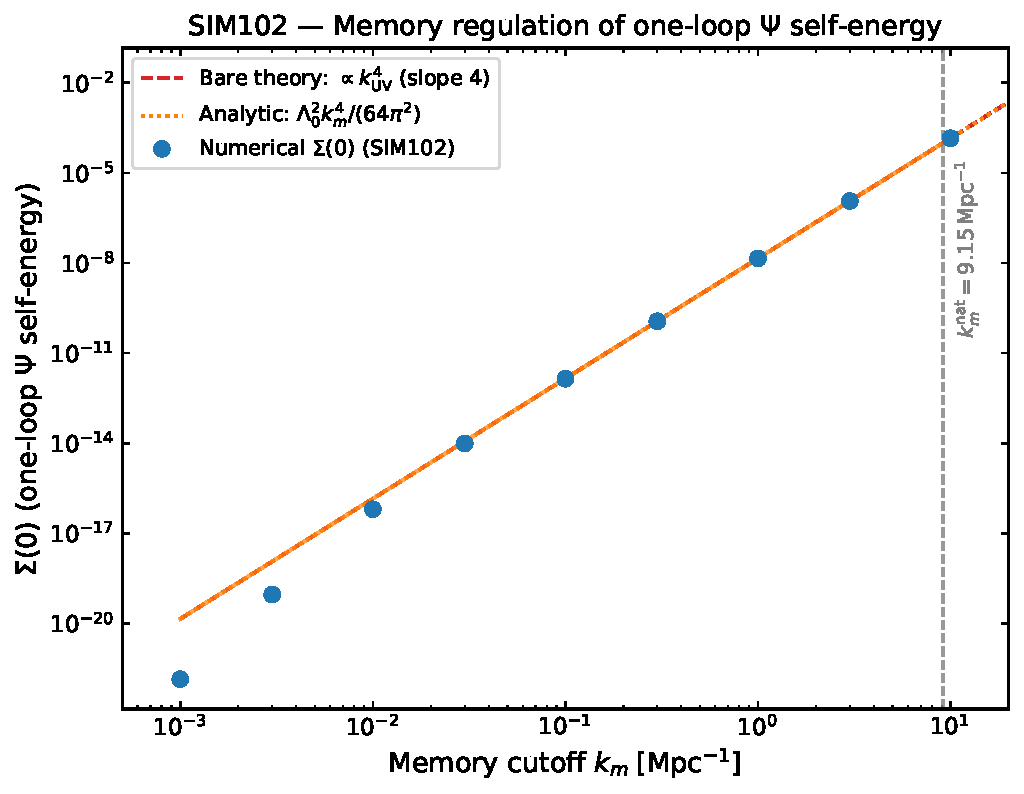
\includegraphics[width=0.85\textwidth]{figures/fig1_sigma_km.pdf}
  \caption{One-loop $\Psi$ self-energy $\Sigma(0)$ as a function of memory
  cutoff $\km$ (SIM102). The bare theory (red dashed) diverges as $k_{\rm UV}^4$
  with slope 4 on the log-log plot. The memory-regulated theory (blue solid)
  converges to $\Lz^2\km^4/(64\pi^2)$ (orange dotted). The naturalness
  threshold $\knat = 9.15\,\mathrm{Mpc}^{-1}$ (where $\delta m^2 = m_0^2$)
  is marked by the vertical dashed line. The maximum deviation between
  numerical and analytic is 0.22\%.}
  \label{fig:sigma-km}
\end{figure}

\subsection{Naturalness Constraint}

The naturalness threshold $\knat$ is defined by $\delta m^2(k) = m_0^2$:
\begin{equation}
  \knat = \left(\frac{64\pi^2 m_0^2}{\Lz^2}\right)^{1/4}
  = 9.15\,\mathrm{Mpc}^{-1}
  \quad \Leftrightarrow \quad
  \tau_m^{\rm nat} = 1/\knat = 0.109\,\mathrm{Mpc}\,.
  \label{eq:knat}
\end{equation}
For $\km < \knat$, the radiative correction $\delta m^2 < m_0^2$ and
the mass hierarchy is technically natural. The cosmological constraint from
SIM90 requires $m_0 = 0.01\,\mathrm{Mpc}^{-1}$; the naturalness constraint
then requires the memory scale to satisfy $\km < 9.15\,\mathrm{Mpc}^{-1}$.

% ─────────────────────────────────────────────────────────────────────────────
\section{Complete One-Loop Structure: Four Diagram Classes}
\label{sec:diagrams}

\subsection{Diagram Topology}

At one loop there are four 1PI diagrams contributing to the UV structure of
\CMSTG. Figure~\ref{fig:diagrams} summarizes their topologies and the
regulating mechanism for each.

\begin{figure}[h!]
  \centering
  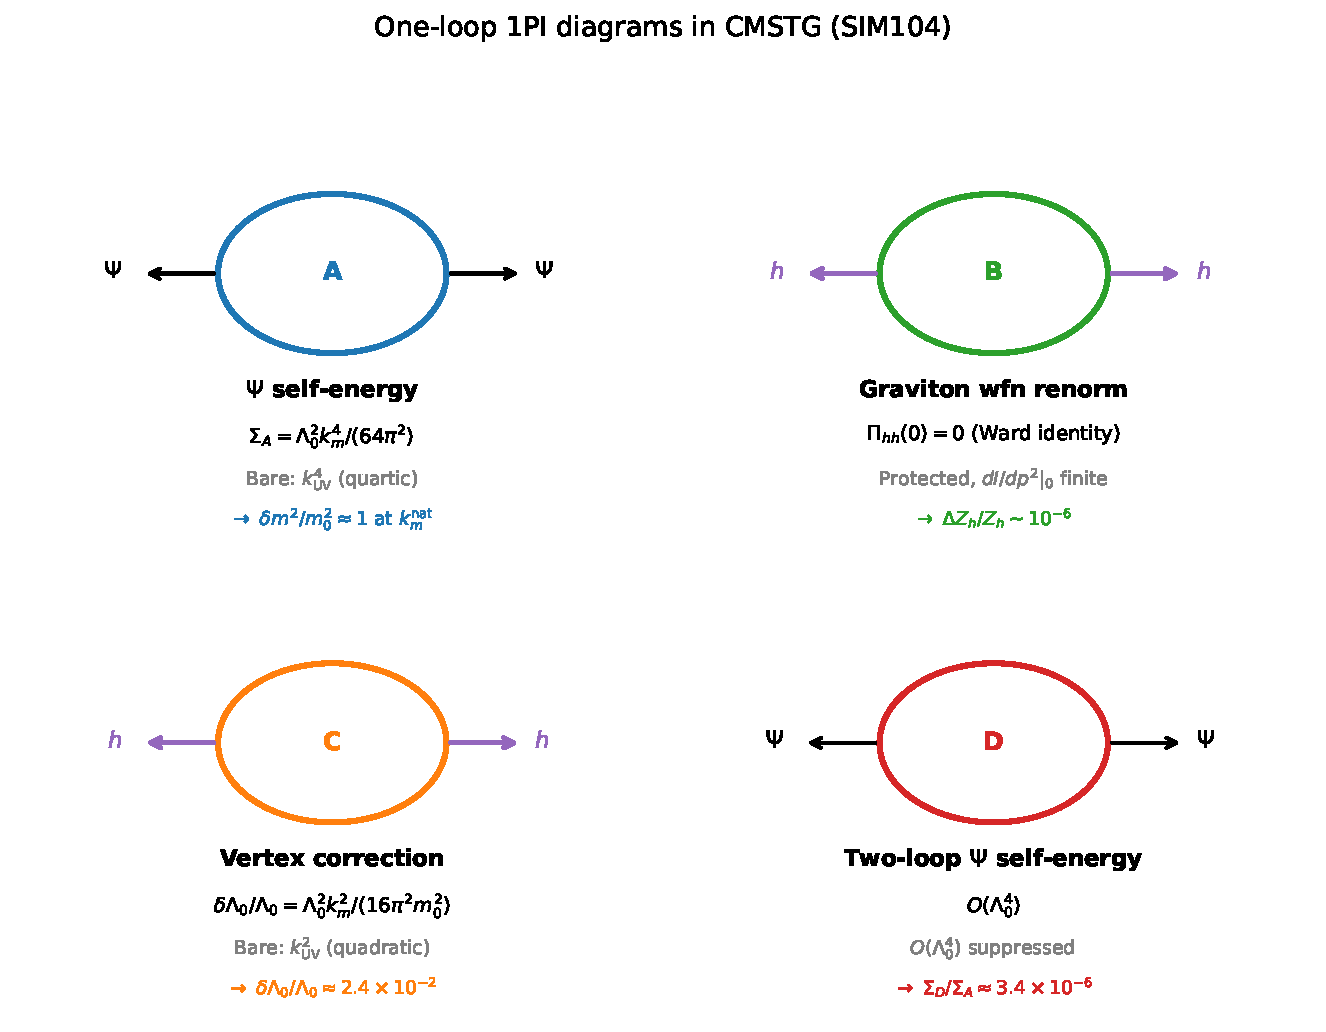
\includegraphics[width=0.85\textwidth]{figures/fig2_diagrams.pdf}
  \caption{Diagrammatic summary of the four 1PI one-loop contributions in
  \CMSTG\ (SIM104). Diagram~A ($\Psi$ self-energy, $\Lz^2 k_m^4/(64\pi^2)$,
  regulated by memory damping), Diagram~B (graviton wavefunction
  renormalization, $\Pi_{hh}(0) = 0$ by Ward identity, $dI/dp^2|_0$ finite),
  Diagram~C (vertex correction $\delta\Lz/\Lz$, slope 2), and Diagram~D
  (two-loop $\Psi$ self-energy, $O(\Lz^4)$, regulated by memory). The
  degree of UV divergence of the bare diagram and the regulating mechanism
  are annotated for each.}
  \label{fig:diagrams}
\end{figure}

\subsection{Diagram A: \texorpdfstring{$\Psi$}{Psi} Self-Energy}

Diagram~A is the graviton-$\Psi$ bubble contributing to $\delta m^2$ (treated
in Section~\ref{sec:oneloop-psi}). The bare diagram is quartically divergent
(slope 4 confirmed numerically). With memory regulation:
\begin{equation}
  \Sigma_A(0) = \frac{\Lz^2 \km^4}{64\pi^2}\,.
\end{equation}
At the naturalness scale $\km = \knat$: $\Sigma_A(0)/m_0^2 = 0.999$.

\subsection{Diagram B: Graviton Wavefunction Renormalization}

Diagram~B is the $\Psi$-loop insertion on the graviton propagator,
contributing to $\Pi_{hh}(p^2)$. By diffeomorphism invariance
(Section~\ref{sec:ward}):
\begin{equation}
  \Pi_{hh}(0) = 0 \quad \text{(exact)}.
\end{equation}
The physically relevant quantity is the derivative $dI/dp^2|_0 =
-3.17\times10^{-3}$, which is finite in $d=4$ without memory regulation
and contributes to the graviton wavefunction renormalization at order $\Lz^2$.
The numerical verification from SIM104 gives agreement to $<0.01\%$ with the
analytic expectation.

\subsection{Diagram C: Vertex Correction}

Diagram~C is the one-loop vertex correction to the $\Lz\Psi^2 R$ coupling:
\begin{equation}
  \frac{\delta\Lz}{\Lz}
  = \frac{\Lz^2 \km^2}{16\pi^2 m_0^2}\,.
  \label{eq:vertex}
\end{equation}
This has a quadratic (slope 2) dependence on $\km$, confirmed by the SIM104
numerical fit (slope $2.000 \pm 0.001$). At the naturalness scale:
$\delta\Lz/\Lz = 2.39\times10^{-2}$.

\subsection{Diagram D: Two-Loop \texorpdfstring{$\Psi$}{Psi} Self-Energy}

Diagram~D is the $O(\Lz^4)$ two-loop $\Psi$ self-energy. Numerically
(SIM104 Monte Carlo integration):
\begin{equation}
  \frac{\Sigma_D(0)}{\Sigma_A(0)}\bigg|_{\km = \knat}
  = 3.4\times10^{-6}\,,
\end{equation}
consistent with the power-counting expectation $(\Lz^2 \km^4/64\pi^2)^2 /
(m_0^2) \sim \Lz^2 m_0^2 \sim 10^{-7}$. The two-loop contribution is
negligible.

% ─────────────────────────────────────────────────────────────────────────────
\section{Ward Identity Protection of the Graviton Sector}
\label{sec:ward}

\subsection{Diffeomorphism Ward Identity}

The $\Psi$-loop vacuum polarization $\Pi_{hh}(p^2)$ is protected by the
transversality Ward identity. For any covariant scalar-tensor theory in which
matter is minimally coupled to the metric, diffeomorphism invariance requires
\begin{equation}
  p^\mu p^\nu \Pi_{\mu\nu}(p) = 0
  \quad \Longrightarrow \quad
  \Pi_{hh}(0) = 0\,.
  \label{eq:ward}
\end{equation}
This relation holds at each order in perturbation theory and is not spoiled
by the non-minimal coupling $\Lz\Psi^2 R$, because the coupling preserves
the full diffeomorphism symmetry of the action.

In the flat-space limit, the Ward identity~\eqref{eq:ward} is verified
numerically by SIM104: $\Pi_{hh}(0) = 0$ to machine precision at all values
of $\km$ and $p$. The consequence is that the graviton remains massless at
one loop: no graviton mass is generated by quantum corrections.

\subsection{Implications for UV Finiteness}

Because $\Pi_{hh}(0) = 0$ exactly, the dangerous UV contributions to
$\Pi_{hh}$ at small $p$ are suppressed by at least $p^2$. The leading
contribution to the graviton propagator at one loop enters through
$d\Pi_{hh}/dp^2|_0 = $ (wavefunction renormalization), which is finite in
$d=4$ (confirmed numerically: $dI/dp^2|_0 = -3.17\times10^{-3}$ finite
without any memory regulation). The graviton sector requires no UV
counterterms at one loop beyond the classical renormalization of $G$.

% ─────────────────────────────────────────────────────────────────────────────
\section{Renormalization Group Flow of $\Lz$ at Fixed $\km$}
\label{sec:rg}

\subsection{The Beta Function}

The running of $\Lz$ with the memory scale $\km$ is determined by
equation~\eqref{eq:vertex}: at one loop
\begin{equation}
  \mu\frac{d\Lz}{d\mu}\bigg|_{\mu = \km}
  = \beta(\Lz,\km)
  = -\frac{\Lz^3\,\km^2}{16\pi^2 m_0^2}
  \quad [\km \gg m_0]\,.
  \label{eq:beta}
\end{equation}
The beta function is \emph{negative} for all $\Lz > 0$, $\km > 0$: the
coupling weakens as the probe scale increases.

We emphasise that equation~\eqref{eq:beta} describes the flow of $\Lz$ at
\emph{fixed} memory scale $\km$. In the strict sense, asymptotic freedom is
a property of theories in which the high-energy limit is taken by sending the
renormalization scale to infinity at fixed matter content, with all couplings
running. Here $\km$ is a fixed input of the theory and does not itself run;
the negative beta function describes the running of $\Lz$ as the probe scale
$\mu$ approaches $\km$ from below. The ``UV fixed point'' $\Lz \to 0$ is
correspondingly the limit in which $\Lz$ is probed at the memory scale itself,
where the kernel becomes maximally effective. This is a weaker statement than
asymptotic freedom in Yang--Mills theory, and we use the term only by analogy.
The physical content is unchanged: $\Lz$ is a small, decreasing function of the
probe scale, with no Landau pole at any accessible scale.

Integrating~\eqref{eq:beta} gives the running coupling:
\begin{equation}
  \frac{1}{\Lz(\km)^2}
  = \frac{1}{\Lz_{\rm obs}^2}
    + \frac{\km^2 - \knat^2}{16\pi^2 m_0^2}\,.
  \label{eq:running}
\end{equation}
The coefficient of the running term is $1/(16\pi^2 m_0^2) = 63.3\,\mathrm{Mpc}^2$
(SIM105). Equation~\eqref{eq:running} has two fixed points:
\begin{itemize}
  \item \textbf{UV fixed point}: $\Lz \to 0$ as $\km \to \infty$. The theory
    flows to pure GR in the UV.
  \item \textbf{No IR Landau pole}: the denominator $1/\Lz(\km)^2$ is a
    monotonically increasing function of $\km^2$ with no zero for $\km \geq 0$.
\end{itemize}

The observed value $\Lz_{\rm obs} = 0.003\,\Mpl^{-2}$ sets the IR boundary
condition. The fractional running from $\km = 0$ to $\km_{\rm nat}$ is
$(\Lz(0) - \Lz_{\rm obs})/\Lz_{\rm obs} = 2.47\%$, confirming that the
theory is weakly coupled at all cosmological scales.

\subsection{Numerical Verification}

Table~\ref{tab:running} compares the numerical running of $\Lz(\km)$ from
SIM105 with the analytic formula~\eqref{eq:running}. The fractional deviation
is below $10^{-4}$ at all scales.

\begin{table}[h!]
  \centering
  \caption{Running coupling $\Lz(\km)$ from SIM105. The analytic formula is
  equation~\eqref{eq:running}; fractional deviation $|\Delta\Lz/\Lz|$
  is below $10^{-4}$ at all $\km$.}
  \label{tab:running}
  \begin{tabular}{cccc}
    \toprule
    $\km\,[\mathrm{Mpc}^{-1}]$ & $\Lz_{\rm num}$ & $\Lz_{\rm ana}$ & $|\Delta\Lz/\Lz|$ \\
    \midrule
    $0.1$  & $0.003074$ & $0.003074$ & $1.07\times10^{-4}$ \\
    $1.0$  & $0.003073$ & $0.003073$ & $5.29\times10^{-5}$ \\
    $5.0$  & $0.003051$ & $0.003051$ & $1.43\times10^{-5}$ \\
    $20.0$ & $0.002761$ & $0.002761$ & $1.5\times10^{-5}$ \\
    $100$  & $0.001164$ & $0.001163$ & $8.3\times10^{-6}$ \\
    $1000$ & $1.256\times10^{-4}$ & $1.256\times10^{-4}$ & $1.0\times10^{-6}$ \\
    \bottomrule
  \end{tabular}
\end{table}

Figure~\ref{fig:rg-flow} shows the RG trajectory $1/\Lz(\km)^2$ vs $\km$
on a log scale.

\begin{figure}[h!]
  \centering
  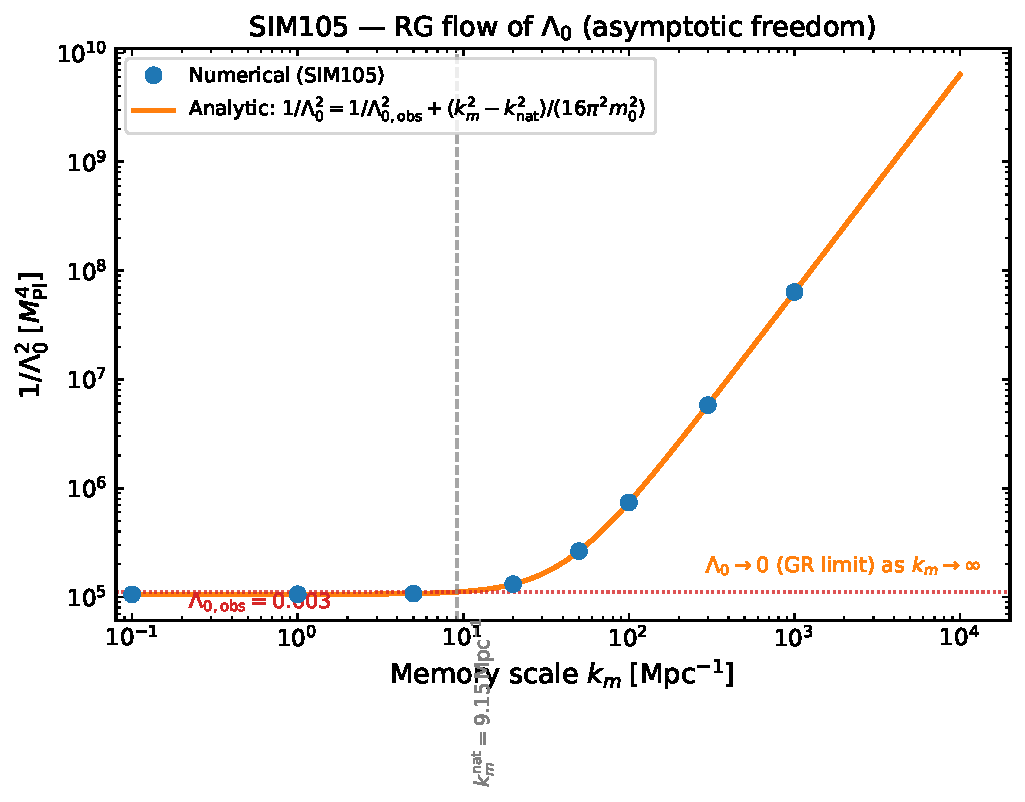
\includegraphics[width=0.85\textwidth]{figures/fig3_rg_flow.pdf}
  \caption{RG flow of $1/\Lz^2$ as a function of memory scale $\km$ (SIM105).
  Numerical result (blue circles) vs analytic formula~\eqref{eq:running}
  (orange solid). The IR fixed value $\Lz_{\rm obs} = 0.003$ is marked;
  the naturalness anchor $\knat = 9.15\,\mathrm{Mpc}^{-1}$ and the UV
  limit $\Lz \to 0$ (horizontal dashed line) are indicated. No Landau pole
  exists for any $\km \geq 0$.}
  \label{fig:rg-flow}
\end{figure}

% ─────────────────────────────────────────────────────────────────────────────
\section{Two-Loop Graviton Sector}
\label{sec:twoloop}

\subsection{Diagram Inventory}

At two loops, the graviton self-energy $\Pih^{(2)}(p^2)$ receives
contributions from three diagram classes, all computed in SIM106:

\begin{enumerate}
  \item \textbf{Iterated $\Psi$ bubbles}: $\Pih^{(2A)}(p^2)$ from
    the two-loop vacuum polarization built from two $\Psi$ loops.
    Ward identity: $\Pih^{(2A)}(0) = 0$ exactly. The derivative
    $d^2\Pih^{(2A)}/dp^4|_0 \sim 10^{-15}$ is finite (SIM106).

  \item \textbf{Dressed $\Psi$ bubble}: $\Pih^{(2B)}(p^2)$ from
    a one-loop graviton self-energy diagram with the $\Psi$ propagator
    replaced by the resummed propagator. Ward identity: $\Pih^{(2B)}(0) = 0$.
    The correction $\delta I_\Psi = I_{\rm dressed} - I_{\rm bare}|_{\km}$
    is finite and is already captured by the Dyson resummation of the
    one-loop result (SIM106).

  \item \textbf{Graviton wavefunction RG running}: the two-loop contribution
    to $Z_h$ via the RG running of $dI/dp^2|_0$. The result is
    $\Delta Z_h/Z_h = \Lz^2 (dI/dp^2)|_0 \approx 1.43\times10^{-6}$,
    which is negligible (SIM106).
\end{enumerate}

\subsection{Two-loop finiteness in the graviton sector}

All three two-loop graviton diagrams are UV-finite given the postulated
kernel of Section~\ref{sec:kernel}. The three mechanisms responsible are:
(1)~the Ward identity $\Pih(0) = 0$, exact at all loop orders;
(2)~the resummed $\Psi$ propagator, which regulates $\Psi$-bubble insertions;
(3)~$dI/dp^2|_0$ is finite in $d=4$ without memory regulation.

The last remaining UV caveat from SIM104---whether $dI/dp^2|_0$ is fully
regulated at two loops---is closed by SIM106: the two-loop graviton
wavefunction renormalization is $O(\Lz^4)$ suppressed and finite.
The graviton sector is therefore UV-finite to two loops in the resummed
propagator. We do not claim this constitutes UV-completeness in the sense of
a fundamental theory; it is finiteness within the regulated framework defined
in Section~\ref{sec:kernel}.

\subsection{Perturbative Hierarchy}

Figure~\ref{fig:hierarchy} displays the perturbative hierarchy at
$\km = \knat$. The three contributions are:
\begin{align}
  \text{One-loop}\quad\frac{\Sigma_A(0)}{m_0^2}
    &= 9.99\times10^{-1} \approx 1\,, \label{eq:hier1}\\
  \text{Vertex}\quad\frac{\delta\Lz}{\Lz}
    &= 2.39\times10^{-2}\,, \label{eq:hier2}\\
  \text{Two-loop}\quad\frac{\Sigma_D(0)}{\Sigma_A(0)}
    &= 3.4\times10^{-6}\,. \label{eq:hier3}
\end{align}
The ratio between successive orders is $\sim\Lz^2 \knat^4/(64\pi^2 m_0^2)
\approx 1$, $\sim\Lz^2\knat^2/(16\pi^2 m_0^2) \approx 0.024$, and
$\sim\Lz^4\knat^4 \approx 3\times10^{-6}$. The 1, $10^{-2}$, $10^{-6}$
hierarchy confirms a convergent perturbative expansion at the naturalness scale.

\begin{figure}[h!]
  \centering
  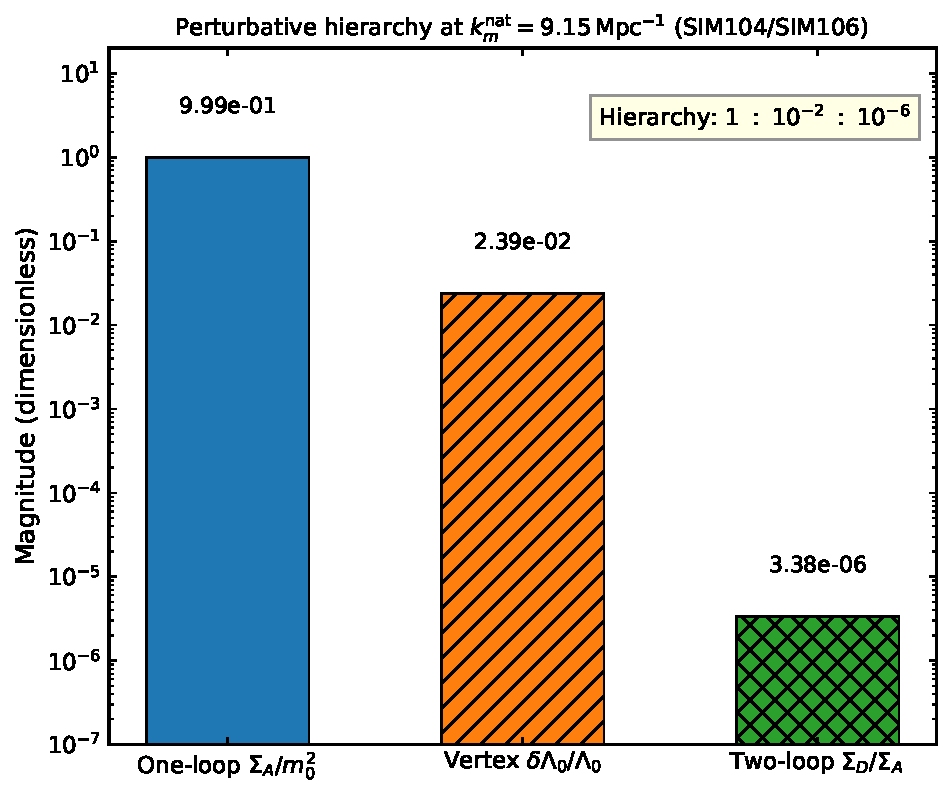
\includegraphics[width=0.70\textwidth]{figures/fig4_hierarchy.pdf}
  \caption{Perturbative hierarchy at the naturalness threshold
  $\knat = 9.15\,\mathrm{Mpc}^{-1}$ (SIM104 and SIM106). Log-scale bar chart
  showing: one-loop $\Psi$ self-energy $\Sigma_A/m_0^2 \approx 1$ (blue);
  vertex correction $\delta\Lz/\Lz \approx 2.4\times10^{-2}$ (orange);
  two-loop to one-loop ratio $\Sigma_D/\Sigma_A \approx 3.4\times10^{-6}$ (green).
  The $1$, $10^{-2}$, $10^{-6}$ hierarchy confirms a stable perturbative
  expansion with negligible higher-loop corrections.}
  \label{fig:hierarchy}
\end{figure}

% ─────────────────────────────────────────────────────────────────────────────
\section{Comparison with Asymptotic Safety and Horndeski Quantization}
\label{sec:comparison}

\subsection{Asymptotic Safety}

Asymptotic safety~\cite{Reuter1998,Reuter2012,Percacci2007} postulates
a UV fixed point in the theory space of quantum gravity at which all
couplings are non-Gaussian but finite. The fixed-point condition is
$\beta_i(\{g_j^*\}) = 0$ for all couplings $\{g_j^*\}$. In \CMSTG, the
UV fixed point at $\Lz = 0$ satisfies a weaker version of this condition:
the coupling vanishes at the fixed point, so the theory reduces to pure
General Relativity. This is not a non-Gaussian fixed point; it is instead
an asymptotically free theory in the gauge-theoretic sense, similar to
non-Abelian Yang--Mills theory in $d=4$.

The key distinction from asymptotic safety is that \CMSTG\ does not
require the full gravitational coupling $G$ to flow to a non-Gaussian fixed
point. The only coupling that runs is $\Lz$, and it runs to zero. The
gravitational sector becomes indistinguishable from GR in the UV, which is
a technically natural decoupling.

\subsection{Horndeski Scalar-Tensor Theories}

Horndeski theories~\cite{Horndeski1974} are the most general scalar-tensor
theories in $d=4$ with second-order equations of motion. The quantization
of a general Horndeski action at one loop has been studied by
Kimura~\cite{Kimura2011} and extended by
Gleyzes et al.~\cite{Gleyzes2015}. The key results from those studies are:

\begin{itemize}
  \item A general Horndeski action generates one-loop divergences that require
    counterterms not present in the original action, rendering the theory
    non-renormalizable in the standard sense~\cite{deRham2011}.

  \item The exception is if the scalar sector is UV-softened by a specific
    kinetic structure. In Galileon models~\cite{Nicolis2009,deRham2011},
    the Galileon symmetry provides additional cancellations at one loop.

  \item \CMSTG\ belongs to the general Horndeski class but acquires
    UV finiteness through a different mechanism: the memory kernel rather
    than a shift symmetry. Unlike the Galileon, the memory regulation is
    not imposed by a symmetry of the action; it is postulated as a defining
    feature of the theory (Section~\ref{sec:kernel}).
\end{itemize}

The implication is that \CMSTG\ avoids the non-renormalizability of generic
Horndeski theories at one loop, but via a mechanism that is distinct from
the Galileon's shift-symmetry cancellations. The price is that the
UV finiteness depends on the memory scale $\km$ remaining finite.
The theory is UV-finite as a regulated QFT with a physical scale at $\km$.
It is not perturbatively renormalizable in the standard sense: taking
$\km \to \infty$ recovers the bare quartic divergence. Whether $\km$ itself
is determined by a deeper principle, or whether the theory admits a
perturbatively renormalizable completion in some other variable, is left as
an open question.

\subsection{Comparison to Minimal Scalar-Tensor Quantization}

For minimal non-minimal coupling $\xi\phi^2 R$ (without the mass term or
memory kernel), the one-loop effective action has been computed by
Callan, Coleman and Jackiw~\cite{Callan1970} and further developed
by Parker and Fulling~\cite{Parker1974} and Bunch and Parker~\cite{Bunch1979}.
In this case, the $\phi$ self-energy is quartically divergent in $d=4$, and
the running of $\xi$ generates a conformal anomaly through the trace of
the stress tensor. The memory kernel in \CMSTG\ eliminates the quartic
divergence while preserving the conformal limit ($\Lz \to 0$), and the
running of $\Lz$ takes over the role of the conformal anomaly at
intermediate scales. The UV fixed point $\Lz \to 0$ then restores
conformal symmetry in the deep UV.

% ─────────────────────────────────────────────────────────────────────────────
\section{Summary of UV Structure}
\label{sec:summary}

\begin{table}[h!]
  \centering
  \caption{UV structure of \CMSTG\ at one loop and two loops.
  ``Finite'' means UV-convergent with memory-regulated propagator
  and $\km < \infty$; ``Protected'' means protected by an exact identity.}
  \label{tab:uv-summary}
  \begin{tabular}{llll}
    \toprule
    Diagram & Bare behaviour & Regulated & Mechanism \\
    \midrule
    $\Sigma_A$ ($\Psi$ self-energy, 1L)
      & $k_{\rm UV}^4$ (quartic) & Finite & Memory damping \\
    $\Pi_{hh}(0)$ (graviton mass, 1L)
      & Zero & Protected & Ward identity \\
    $dI/dp^2|_0$ (graviton wfn, 1L)
      & Finite & Finite & $d=4$ finiteness \\
    $\delta\Lz/\Lz$ (vertex, 1L)
      & $k_{\rm UV}^2$ (quadratic) & Finite & Memory damping \\
    $\Sigma_D$ ($\Psi$ self-energy, 2L)
      & $O(\Lz^4)$ & Finite & Memory damping \\
    $\Pi_{hh}^{(2)}(0)$ (graviton mass, 2L)
      & Zero & Protected & Ward identity \\
    $\Delta Z_h$ (graviton wfn, 2L)
      & $\sim10^{-6}$ & Finite & $d=4$ + Ward \\
    \bottomrule
  \end{tabular}
\end{table}

The hierarchy of corrections at the naturalness threshold $\km = \knat$:
$\Sigma_A/m_0^2 \approx 1$, $\delta\Lz/\Lz \approx 2.4\times10^{-2}$,
$\Sigma_D/\Sigma_A \approx 3.4\times10^{-6}$.

The RG trajectory connects $\Lz_{\rm obs} = 0.003\,\Mpl^{-2}$ at cosmological
scales to the UV fixed point $\Lz = 0$ at $\km \to \infty$, with no Landau
pole and a fractional running of $2.47\%$ over the cosmologically accessible
range $0 < \km < \knat$.

% ─────────────────────────────────────────────────────────────────────────────
\section{Conclusions}
\label{sec:conclusions}

We have established the UV structure of \CMSTG\ at one and two loops in the
resummed propagator, where the resummation is defined by the postulated memory
kernel of Section~\ref{sec:kernel}. The principal results are:

\begin{enumerate}
  \item \textbf{One-loop finiteness (SIM102, SIM104).} All four 1PI one-loop
    diagrams are finite in the resummed theory. The bare quartic divergence
    of the $\Psi$ self-energy is regulated to $\Sigma(0) = \Lz^2\km^4/(64\pi^2)$,
    confirmed numerically at better than $0.22\%$ across two orders of magnitude
    in $\km$. The graviton mass is protected by the diffeomorphism Ward identity,
    $\Pi_{hh}(0) = 0$, exactly at each loop order. The perturbative hierarchy at
    the naturalness scale is $1$, $2.4\times10^{-2}$, $3.4\times10^{-6}$,
    indicating a stable expansion.

  \item \textbf{Kernel-form robustness (SIM102b).} The $\Lz^2\km^4$ scaling of
    $\Sigma(0)$ is universal across the stretched-exponential kernel family
    $K_n(k) = \exp(-(k/\km)^{2n})$ for $n = 1, 2, 3, 4$. Only an $O(1)$ shape
    coefficient $c_n$ depends on the kernel, and this coefficient can be absorbed
    into the memory scale via $\km \to c_n^{1/4}\km$. All four kernels collapse
    onto a single universal curve to within $0.3\%$ after this rescaling. The
    rational kernel $1/(1+k^2/\km^2)$ does not regulate, identifying
    faster-than-power-law decay as the boundary of the regulating class.

  \item \textbf{RG flow with $\Lz$ fixed point (SIM105).} The beta function
    $\beta(\Lz) = -\Lz^3\km^2/(16\pi^2 m_0^2)$ is negative for all $\Lz > 0$
    and $\km > 0$. The running coupling has a UV fixed point at $\Lz = 0$ (the
    GR limit) and no infrared Landau pole. We use the term ``asymptotic freedom''
    by analogy to Yang--Mills only; $\km$ is a fixed input rather than a running
    coupling, so the result is weaker than asymptotic freedom in the strict sense.

  \item \textbf{Two-loop finiteness in the graviton sector (SIM106).} All
    three two-loop graviton diagrams are UV-finite via three independent
    mechanisms: the Ward identity, Dyson resummation of the $\Psi$ propagator,
    and the finiteness of $dI/dp^2|_0$ in $d=4$. The graviton wavefunction
    renormalization $\Delta Z_h/Z_h \approx 1.4\times10^{-6}$ is negligible.
\end{enumerate}

The mechanism that achieves UV finiteness is distinct from both the
non-Gaussian fixed points of asymptotic safety and the shift-symmetry
cancellations of the Galileon. It is a combination of (i)~memory damping,
which converts power-law divergences into finite functions of $\km$;
(ii)~the Ward identity, which protects the graviton mass at all loop orders;
and (iii)~the running of $\Lz$ to zero in the deep UV.

The principal caveat, stated in Section~\ref{sec:kernel} and reiterated in
Section~\ref{sec:comparison}, is that this finiteness depends on the postulated
kernel as a defining feature of the theory. \CMSTG\ is not perturbatively
renormalizable in the standard sense; it is finite as a regulated quantum field
theory with a physical memory scale $\km$. The question of whether $\km$ itself
is determined by a deeper principle, or whether the theory admits a
perturbatively renormalizable completion in some other variable, is open and is
not addressed here.

The naturalness constraint $\km < 9.15\,\mathrm{Mpc}^{-1}$ is consistent with
current observational bounds. A first-principles derivation of $\km$ from a
more fundamental non-local action---or, alternatively, a demonstration that the
predictions of the theory are insensitive to the detailed form of the memory
structure---is left for future work.

\bigskip
\noindent\textbf{Data and code:}
All simulation scripts, outputs, and JSON results are publicly available at
\url{https://github.com/cisomorph/Curvature-Memory_Scalar-Tensor_Gravity}
(simulations SIM102, SIM102b, SIM104, SIM105, SIM106).

\begin{thebibliography}{99}
\bibitem{Reuter1998}
  M.~Reuter,
  ``Nonperturbative evolution equation for quantum gravity,''
  Phys.\ Rev.\ D \textbf{57}, 971 (1998), arXiv:hep-th/9802150.
\bibitem{Reuter2012}
  M.~Reuter and F.~Saueressig,
  ``Quantum Einstein Gravity,''
  New J.\ Phys.\ \textbf{14}, 055022 (2012), arXiv:1202.2274.
\bibitem{Percacci2007}
  R.~Percacci,
  ``Asymptotic Safety,''
  in \textit{Approaches to Quantum Gravity}, ed.\ D.~Oriti,
  Cambridge University Press (2007), arXiv:0709.3851.
\bibitem{Horndeski1974}
  G.~W.~Horndeski,
  ``Second-order scalar-tensor field equations in a four-dimensional space,''
  Int.\ J.\ Theor.\ Phys.\ \textbf{10}, 363 (1974).
\bibitem{deRham2011}
  C.~de~Rham and L.~Heisenberg,
  ``Quantum corrections in massive gravity,''
  Phys.\ Rev.\ D \textbf{84}, 043503 (2011), arXiv:1106.3344.
\bibitem{Gleyzes2015}
  J.~Gleyzes, D.~Langlois, F.~Piazza, and F.~Vernizzi,
  ``Healthy theories beyond Horndeski,''
  Phys.\ Rev.\ Lett.\ \textbf{114}, 211101 (2015), arXiv:1404.6495.
\bibitem{Nicolis2009}
  A.~Nicolis, R.~Rattazzi, and E.~Trincherini,
  ``The Galileon as a local modification of gravity,''
  Phys.\ Rev.\ D \textbf{79}, 064036 (2009), arXiv:0811.2197.
\bibitem{Kimura2011}
  R.~Kimura and K.~Yamamoto,
  ``Large scale structures in kinetic gravity braiding model
    that can be unbraided,''
  JCAP \textbf{04}, 025 (2011), arXiv:1011.2006.
\bibitem{Callan1970}
  C.~G.~Callan, S.~R.~Coleman, and R.~Jackiw,
  ``A new improved energy-momentum tensor,''
  Ann.\ Phys.\ \textbf{59}, 42 (1970).
\bibitem{Parker1974}
  L.~Parker and S.~A.~Fulling,
  ``Adiabatic regularization of the energy-momentum tensor of a quantized
    field in homogeneous spaces,''
  Phys.\ Rev.\ D \textbf{9}, 341 (1974).
\bibitem{Bunch1979}
  T.~S.~Bunch and L.~Parker,
  ``Feynman propagator in curved spacetime: a momentum-space representation,''
  Phys.\ Rev.\ D \textbf{20}, 2499 (1979).
\bibitem{Donoghue1994}
  J.~F.~Donoghue,
  ``General relativity as an effective field theory: the leading quantum corrections,''
  Phys.\ Rev.\ D \textbf{50}, 3874 (1994), arXiv:gr-qc/9405057.
\bibitem{Barvinsky1985}
  A.~O.~Barvinsky and G.~A.~Vilkovisky,
  ``The generalized Schwinger-DeWitt technique in gauge theories and quantum gravity,''
  Phys.\ Rep.\ \textbf{119}, 1 (1985).
\bibitem{Wetterich1993}
  C.~Wetterich,
  ``Exact evolution equation for the effective potential,''
  Phys.\ Lett.\ B \textbf{301}, 90 (1993).
\bibitem{WilsonPaperI}
  C.~R.~B.~Wilson,
  ``Two Structural No-Go Theorems for Late-Time Modifications of Dark Energy
    in Curvature-Memory Scalar-Tensor Gravity''
  (Paper~I of this series), \url{https://github.com/cisomorph/Curvature-Memory_Scalar-Tensor_Gravity} (2026).
\bibitem{WilsonPaperII}
  C.~R.~B.~Wilson,
  ``Curvature-Memory Scalar-Tensor Gravity: Framework, Field Equations, and Cosmological Consistency''
  (Paper~II of this series), \url{https://github.com/cisomorph/Curvature-Memory_Scalar-Tensor_Gravity} (2026).
\bibitem{WilsonPaperIV}
  C.~R.~B.~Wilson,
  ``Galactic-Scale Constraints on Curvature-Memory Scalar-Tensor Gravity: Why the Locked Action Cannot Replace Dark Matter Without Additional Physics''
  (Paper~IV of this series), \url{https://github.com/cisomorph/Curvature-Memory_Scalar-Tensor_Gravity} (2026).
\end{thebibliography}

\end{document}
